\documentclass[10pt,a4paper]{article}
\usepackage[utf8]{inputenc}
\usepackage{amsmath}
\usepackage{amssymb}
\usepackage{graphicx}
\usepackage{amsfonts}
%\usepackage[spanish]{babel}

%Ruta de imágenes
\graphicspath{{images/}}

\title{Laboratorio de Diseño Digital Moderno Experimento No. 13 Memoria RAM}
\author{}
\date{\today}

\begin{document}
	\maketitle
	
	\section{Creación de RAM}
	\subsection{Compilación}
	\begin{center}
		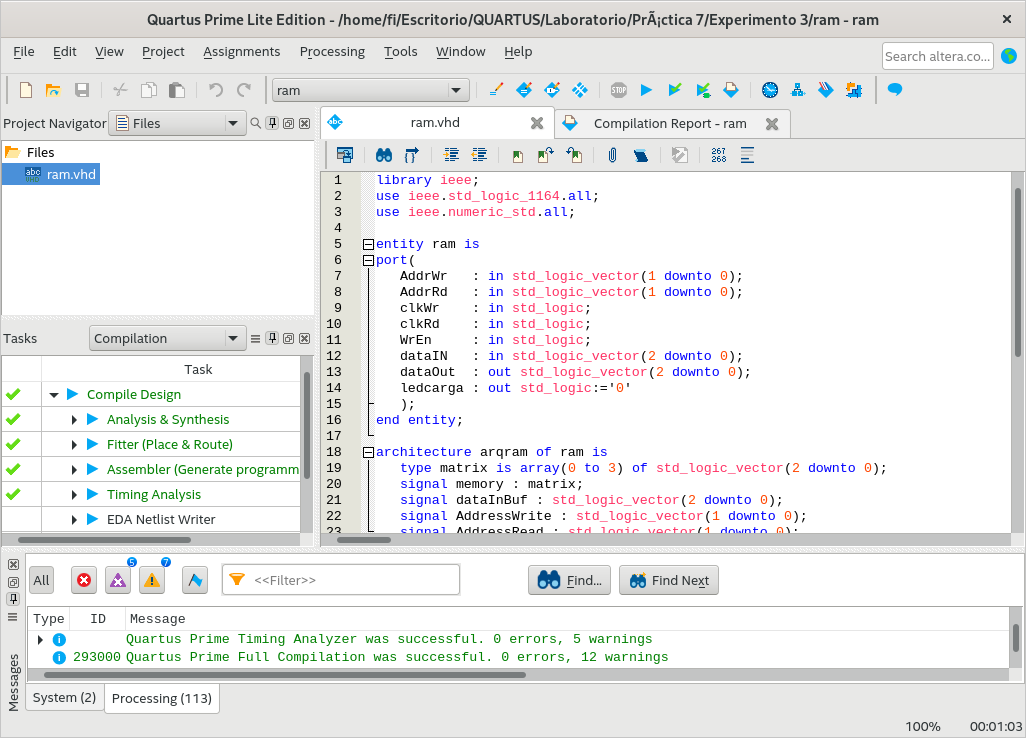
\includegraphics[scale=0.35]{Compilacion.png}
	\end{center}
	
	\subsection{Diagrama RTL}
	\begin{center}
		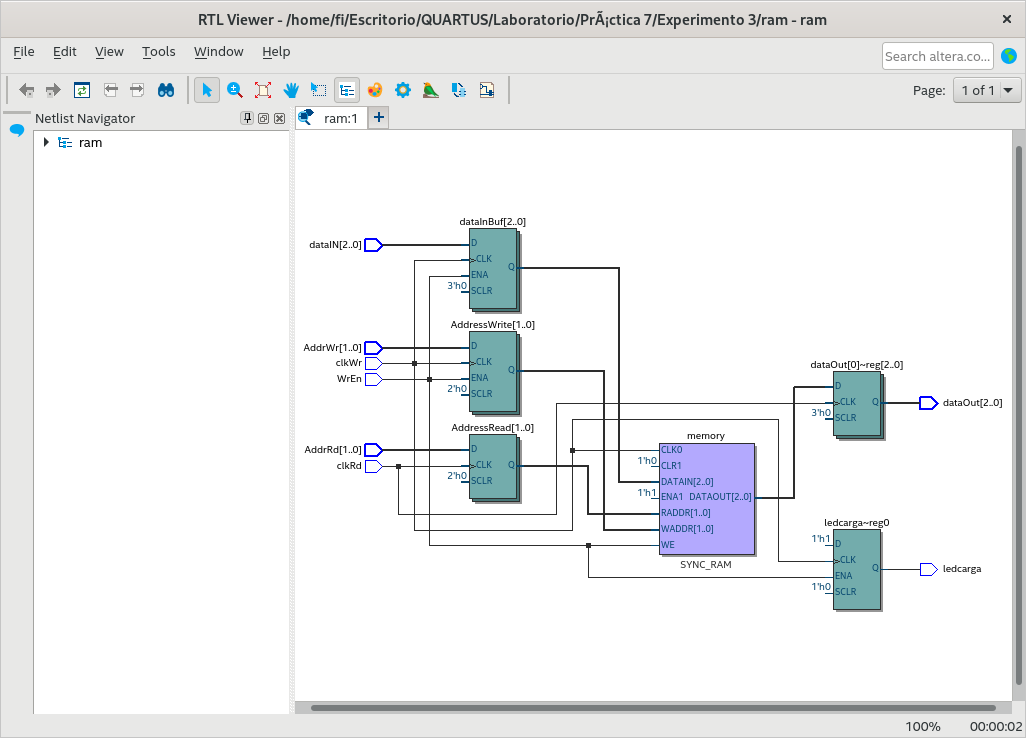
\includegraphics[scale=0.35]{RTL.png}
	\end{center}
	
	\subsection{Simulación}
	\begin{center}
		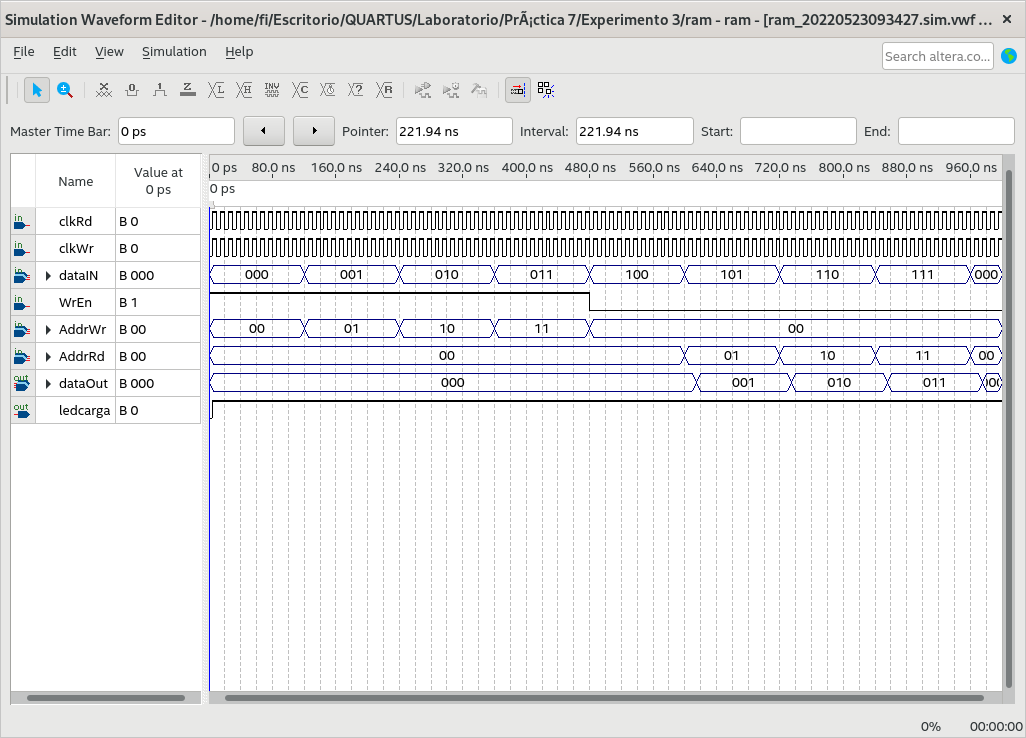
\includegraphics[scale=0.35]{Simulacion.png}
	\end{center}
	
	\subsection{Asignación de pines}
	\begin{center}
		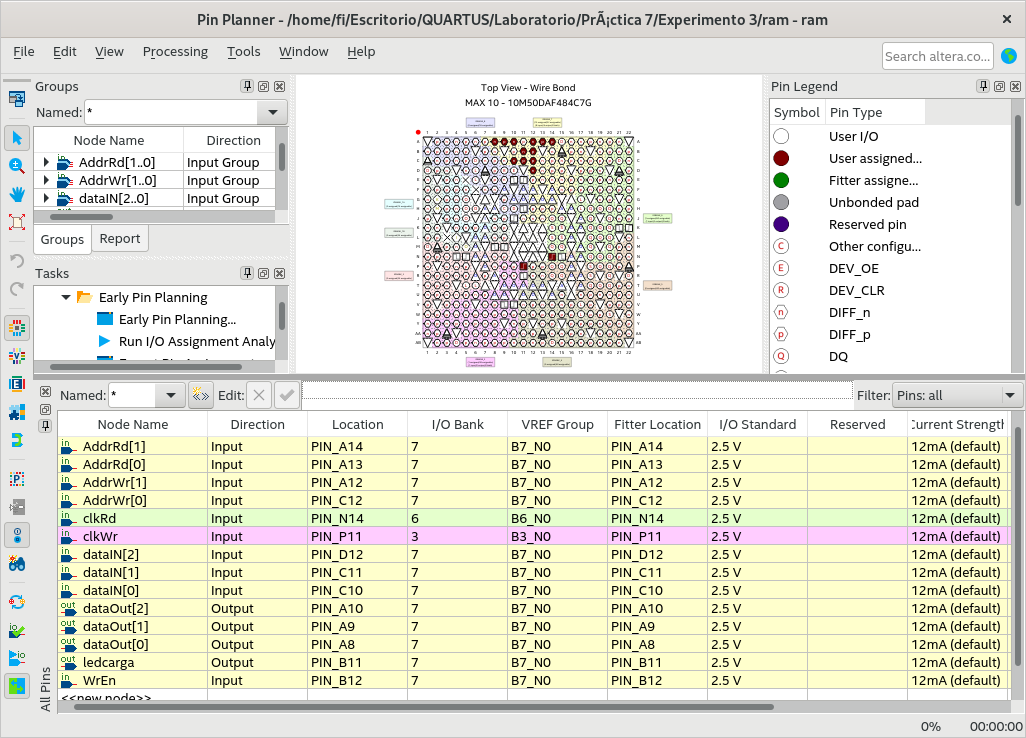
\includegraphics[scale=0.35]{Pines.png}
	\end{center}
	
	\subsection{Descarga a tarjeta}
	\begin{center}
		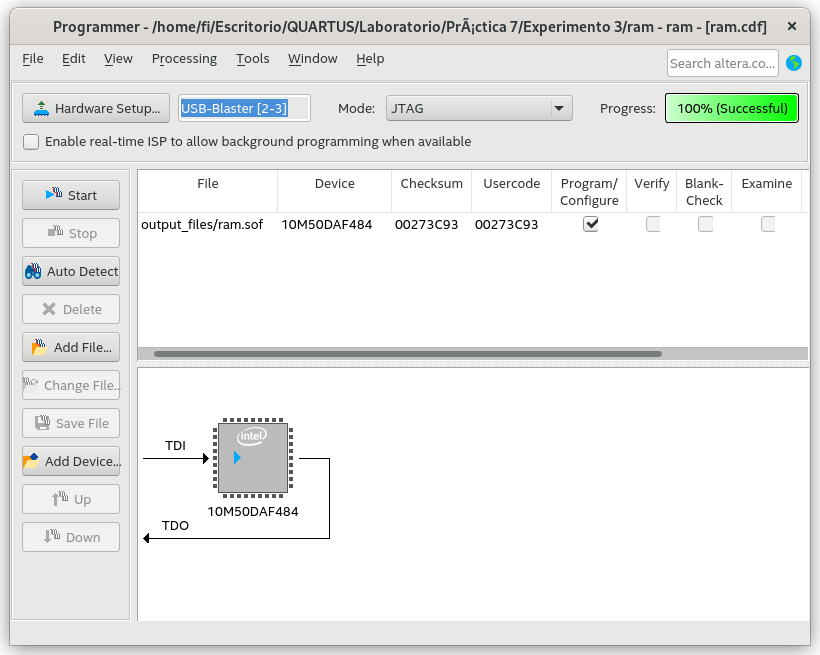
\includegraphics[scale=0.35]{Descarga.png}
	\end{center}
	
\end{document}